% A template for a report in LaTeX
% author: team MOOC Mathematical modelling basics
% June 2017


% Always compile 3 times, to get the table of contents and references right.
\documentclass[11pt, a4paper, twoside]{report} 
\setcounter{tocdepth}{4}
\setcounter{secnumdepth}{4}
\usepackage{float}

\usepackage[margin=4cm]{geometry}   % For smaller margins
\usepackage{color}          % So you can use colors
\usepackage{amsmath, amsfonts, amssymb} % For all kinds of math symbols
\usepackage{graphicx}	    % Package to include photos and graphs 
\usepackage{float}          % Helps in positioning floats
\usepackage[justification=centering]{caption}  % To center the captions of graphs
\usepackage{url}
\setlength{\parindent}{0pt} % When you do not want indentation for your paragraphs.
\setlength{\parskip}{11pt}  % For space between paragraphs.

\begin{document} % Here the document starts

%--Title page--------A little bit more complex than the rest....

\begin{titlepage}

\newcommand{\HRule}{\rule{\linewidth}{0.5mm}} % Defines a new command for the horizontal lines

\begin{center}
~\vspace{1cm}  % vertical space

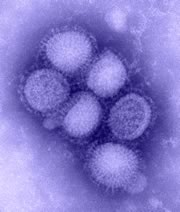
\includegraphics[width=\linewidth, height=13cm]{B00528_H1N1_flu_blue_sml}

\HRule \\[0.4cm] %Horizontal line and [0.4cm] extra spacing
\textsc{\LARGE Epidemic model for influenza A (H1N1)}\\[0.5 cm] % Title of report 
\textsc{\Large Modeling the outbreak of the pandemic in Kolkata, West Bengal, India, 2010}\\[0.1 cm] % Subtitle 
\HRule \\[1.5cm]


\begin{minipage}{0.4\textwidth}
    \large
    \begin{center} 
    \textsc{Sandipan Dey} \\ %Name and country of person 1
    \textsc{India}       
    \end{center}
\end{minipage}
~

{\large \today}\\ % \today automatically gives todays date
\end{center}
\end{titlepage}

% This is the end of the titlepage ----------------------------------------------

~

% Summary ----------------------------------------------

\chapter*{Summary} 
\addcontentsline{toc}{chapter}{Summary} 
In this report, the spread of the pandemic influenza A (H1N1) that had an outbreak in Kolkata, West Bengal, India, 2010 is going to be simulated. The basic epidemic SIR model will be used, it describes three populations: a susceptible population, an infected population, and a recovered population and assumes the total population (sum of these 3 populations) as fixed over the period of study. There are two parameters for this model: namely the attack rate ($\beta$) per infected person per day through contacts and the recovery rate ($\alpha$). 

Initially there will be a small number of infected persons in the population. Now the following questions are to be answered with the simulation / analysis:

\begin{enumerate}
\item Whether the number of infected persons increase substantially, producing an epidemic, or the flue will fizzle out. 
\item Assuming there is an epidemic, how will it end? Will there still be any susceptibles left when it is over? 
\item How long will the epidemic last?
\end{enumerate}

Euler method will be primarily used to solve the system of differential equations for SIR model and compute the equilibrium points (along with some analytic solution attempts for a few simplified special cases). Here are the conclusions obtained from the simulations:

\begin{enumerate}
\item When the recovery rate $\alpha$ is $\approx 0$ or very low compared to the attack rate $\beta$, the flu will turn out to be an epidemic and the entire population will be infected first (the higher $\beta$ is the quicker the epidemic). 
\item When there is an epidemic, it will eventually end in the equilibrium point with $0$ infected population, how fast it reaches the equilibrium depends upon the recovery rate (the higher $\alpha$ is the quicker the infection removal).
\item The time to reach the equilibrium can be computed using Euler method, it depends on the parameters $\alpha$ (the higher the quicker) and $\beta$ (the higher the quicker) and the initial infected populated size $I(0)$ (the higher the quicker).
\item If there the recovery rate $\alpha$ is much higher than the attack rate  $\beta$, even when the equilibrium is reached the susceptible population size may be non-zero. 
\end{enumerate}


% Table of contents ----------------------------------------------

\newpage
\tableofcontents %The table of contents is made. You have to compile 3 times to get it right.

% List of variables ----------------------------------------------

\chapter*{List of variables}
\addcontentsline{toc}{chapter}{List of variables}

\begin{table}[H]

\begin{tabular}{| l | l | l |}

\hline
Variable &  Description & Unit \\ \hline
t & time & day \\ \hline
S(t) & the size of \textbf{susceptible} population at time $t$,  & person \\   
      & who are not infected but could become infected &  \\ \hline
I(t) & the size of \textbf{infected} population at time $t$, individuals  & person \\       & that have / can transmit flu to susceptible population & \\ \hline
R(t) & the size of \textbf{removed} population at time $t$, individuals  & person \\
     & that can not become infected / transmit flu to others &  \\ \hline
$\alpha$ & the \textbf{recovery rate}, the rate with which an infected & $[day]^{-1}$ \\
     & recovers and moves into the removed state &   \\ \hline
$\beta$ & the \textbf{attack rate}, \textbf{fraction} of \textbf{susceptible-infected} & $[person]^{-1}[day]^{-1}$ \\ 
     & contacts results in a new infection, i.e., \textbf{proportion} & \\  
     & of disease-spreading contacts made by each infected &  \\ 
     & individual per day & \\
\hline

\end{tabular}

\end{table}

% --MAIN TEXT-------------------------------------
% --Introduction-------------------------------------

\chapter{Introduction} %Numbered chapters are added to the table of contents automatically.
In 2010, the pandemic influenza A (H1N1) had an outbreak in Kolkata, West Bengal, India. An increased number of cases with influenza like illness (ILI) were reported in Greater Kolkata Metropolitan Area (GKMA) during July and August 2010, as stated in \cite{bib:ijmr}. The main motivation for this research project will be to understand the spread of the pandemic, compute the equilibrium points and find the impact of the initial values of the infected rate and the attack / recovery rate parameters on the spread of the epidemic, using simulations using the basic epidemic SIR model.

Euler method will be primarily used to solve the system of differential equations for SIR model and compute the equilibrium points. First a few simplified special cases will be considered and both analytic and numerical methods (with Euler method) will be used to compute the equilibrium points. Then the solution for the generic model will be found. 

The chapter 1 describes all the methods used along with the results obtained for simplified special cases along with the generic model. Different combinations of the parameter values (and the initial values of the variables) will be used to understand the impact of the change of the values in parameters / initial values of the variables. The conclusions chapter discusses the conclusions obtained from the simulations. And finally the bibliography contains the references for the external sources, followed by appendix, that contains derivation of long analytic solutions / long tables.


% --Chapter-------------------------------------

\chapter{SIR Epidemic model}


The SIR model is an epidemiological model that computes the theoretical number of people infected with a contagious illness in a closed population over time. One of the basic one strain SIR models is Kermack-McKendrick Model. The Kermack-McKendrick Model is used to explain the rapid rise and fall in the number of infective patients observed in epidemics.

It assumes that the population size is \textbf{fixed} (i.e., no births, no deaths due to disease nor by natural causes), incubation period of the infectious agent is instantaneous, and duration of infectivity is the same as the length of the disease. It also assumes a completely homogeneous population with no age, spatial, or social structure.

The following figure \ref{fig:virus} shows an electron microscope image of the re-assorted H1N1 influenza virus photographed at the CDC Influenza Laboratory. The viruses are $80-120$ nm in diameter \cite{bib:wiki}.

\begin{figure}[H]
\centering
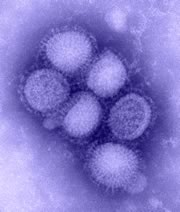
\includegraphics[width=\linewidth]{B00528_H1N1_flu_blue_sml.jpg}
\caption{Electron microscope image of the re-assorted H1N1 influenza virus photographed at the CDC Influenza Laboratory \cite{bib:virus}}
\label{fig:virus}
\end{figure}


\section{Basic Mathematical Model}
\label{section:mathmodel}

The starting model for an epidemic is the so-called SIR model, where S stands for susceptible population, the people that can be infected. I is the already infected population, the people that are contagious, and R stands for the recovered population, people who are not contagious any more. 

\subsection{Differential Equations}

The \textbf{SIR} model can be defined using the following ordinary differential equations \ref{eq:sir}:


\begin{equation}
\left\{   % The left brace
\begin{array}{rcl} 
\dfrac{dS(t)}{dt} & = & -\beta S(t)I(t)\\
\\
\dfrac{dI(t)}{dt} & = & \beta S(t)I(t) - \alpha I(t) \\
\\
\dfrac{dR(t)}{dt} & = & \alpha I(t) \\
\end{array}
\right. 
\label{eq:sir}
\end{equation}

\begin{itemize}
 \item The terms $\dfrac{dS}{dt},\;\dfrac{dI}{dt},\;\dfrac{dR}{dt}$ in the differential equations indicate the rate of change of the susceptible population size, the infected population size and the recovered population size, respectively. 
 \item The term $\beta$ and $\alpha$ indicate the attack rate (number of susceptible persons get infected per day) and the recovery rate of the flu (inverse of the number of days a person remains infected), respectively. 
 \item High value of $\alpha$ means a person will be infected by the flu for less number of days and high value of $\beta$ means that the epidemic will spread quickly.
 \item Also, as can be seen from below, from the differential equations it can be shown that the population ($S + I + R$) is assumed to be constant.
 
 \begin{equation*}
 \begin{array}{ll} 
 \dfrac{dS}{dt}+\dfrac{dI}{dt}+\dfrac{dR}{dt} & \\\\
 = -\beta S(t)I(t) + \beta S(t)I(t) - \alpha I(t) + \alpha I(t) & (by\; \ref{eq:sir}) \\\\
 = 0 & \\\\
 \Rightarrow \dfrac{d}{dt}(S+I+R) = 0 & \\\\
 \Rightarrow S+I+R = constant & 
 \end{array}
 \end{equation*}
\end{itemize}

\subsection{Collected data, units and values for the constants}

\begin{itemize}
\item As can be seen from the following figure \ref{fig:kmc}, the focus of this analysis will be limited to the population in Kolkata Metropolitan Corporation (\textbf{KMC}, XII) area where the population can be assumed to be $\approx 4.5$ million or 4500 thousands, as per \cite{bib:kmc}. 
\item \textbf{Units} 
\begin{itemize} 
\item All population ($S, I, R$) units will be in \textit{thousands persons} (so that total population $N$ = 4500). 
\item As can be derived from the differential equations \ref{eq:sir}, the unit of $\beta$ will be in \textit{$10^{-6}$ $[persons]^{-1}[day]^{-1}$}  ($\beta=25$ will mean $25$ \textit{persons in a million} gets infected by susceptible-infected contact \textit{per infected persoon} \textit{per day}).
\item Similarly, the units of $\alpha$ will be in \textit{$10^{-3}$ / day} ($\alpha=167$ will mean $167 \times 10^{-3}$ /day  gets recovered from the flu \textit{per day}).
\end{itemize}
\item The attack rate is 20-29/100000 and the number of days infected (i.e. the inverse of recovery rate) = $5-7$ days on average (with a few exceptions), as per \cite{bib:ijmr}. 
\item Typical values for $\beta$ and $\alpha$ can be assumed to be $25$ /person / day and $\frac{10^3}{6} \approx 167$ / day, respectively. 
\end{itemize}

\begin{figure}[H]
\centering
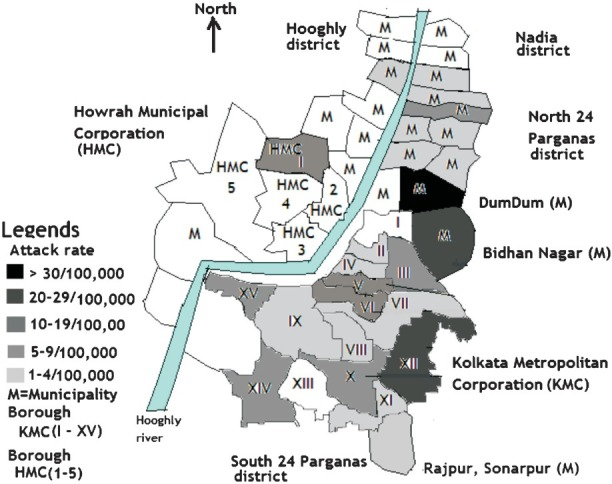
\includegraphics[width=\linewidth]{IJMR-135-529-g004.jpg}
\caption{Attack rate per 100,000 population of ILI by borough of Kolkata Metropolitan Corporation \cite{bib:ijmr}}
\label{fig:kmc}
\end{figure}


\section{Simplified Model 1 (with $\alpha=0$)}
\label{section:simplemathmodel1}

\begin{itemize}

\item Let us start with a simplified model: let us assume that $\alpha=0$ (/ day) and that $R=0$, so once infected, a person stays contagious for ever. Because $S(t)+I(t)+R(t)=S(t)+I(t)=N$ is constant (since population size $N$ is fixed),  $S(t)$ can be eliminated and a single differential equation in just $I(t)$ is obtained as shown in the equation below \ref{eq:simsir}. 

\begin{equation}
\begin{array}{rcl} 
\dfrac{dI(t)}{dt} & = & \beta I(t)(N-I(t))
\end{array}
\label{eq:simsir}
\end{equation}

\item Also, let the (fixed) population size $N=4500=S(0)+I(0)$, (in thousand persons), \textit{initially} the number of persons \textit{infected} $=I(0)=1$ (in thousand persons) and \textit{susceptible} $S(0)=N-I(0)=4499$ (in thousand persons), respectively. Let $\beta=25 \times 10^{-6}$ /persons / day) to start with.

\end{itemize}

\subsection{Analytic Solution}
\label{subsection:analytic}

\begin{itemize}

\item The analytic solution can be found by following the steps shown in the \textit{Appendix A} and the final solution is shown in the below equations \ref{eq:simsira}:

\begin{equation}
\begin{array}{rcl} 
I(t) &=& \dfrac{N}{1+e^{C-\beta N t}} \\
     & & where \;\; C = ln\left(\frac{N}{I(0)}-1\right)
\end{array}
\label{eq:simsira}
\end{equation}

\item The following figure \ref{fig:anl1} shows the \textbf{logistic} (\textbf{bounded}) growth in $I(t)$ (\textbf{in thousands persons}) w.r.t. the time (\textbf{in days}) for different values of attack rate $\beta \times 10^{-6}$ (/ person / day). As expected, the higher the attack rate, the quicker all the persons in the population become infected. 

\begin{figure}[H] % [h!]
\centering
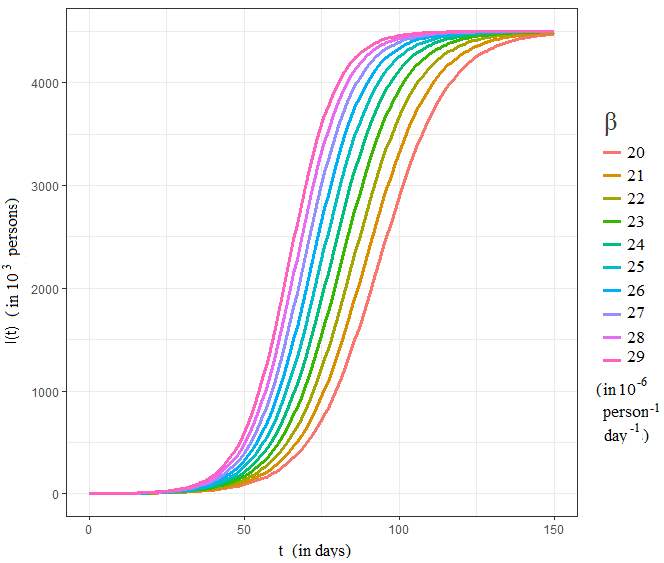
\includegraphics[width=\linewidth]{r1_0.png}
\caption{Growth of the number of infected persons}
\label{fig:anl1}
\end{figure}

\end{itemize}

\subsection{Finding the equilibrium points for $I$} 
\label{subsection:eq}

\begin{itemize} 

\item The equilibrium points are the points where the rate of change in $I$ is \textit{zero}, the points that satisfy the following equation 
\begin{align*}
\dfrac{dI(t)}{dt}=0\\
\Rightarrow \beta I(t)(N-I(t))=0 \\
\Rightarrow I(t)=0, N 
\end{align*}

\item Considering a small \textit{neighborhood} of the equilibrium point at $I=0$, it can be seen from the figure \ref{fig:seq} that whenever $I>0,\; \dfrac{dI}{dt}>0$, so $I$ increases and goes away from the equilibrium point. \item Hence, the equilibrium point at $I=0$ is \textbf{unstable}.

\item At $I=N=4500$ (in thousand persons) it is a \textbf{stable} equilibrium. As can be seen from the following figure \ref{fig:seq}, in a small \textit{neighborhood} of the equilibrium point at $I=4500$, it always increases / decreases towards the equilibrium point.

\item In a small $\epsilon > 0$ \textit{neighborhood} at $I=4500$ (in thousand persons),
\begin{enumerate}
    \item $\dfrac{dI}{dt} > 0$, so $I$ increases when $I <= 4500 - \epsilon$. \item $\dfrac{dI}{dt} > 0$, so $I$ decreases when $I >= 4500 + \epsilon$ .
\end{enumerate}

\item The same can be observed from the \textit{direction fields} from the figure \ref{fig:dir}. 

\item Hence, the equilibrium at $I=4500$ is \textbf{stable}.

\begin{figure}[H]
\centering
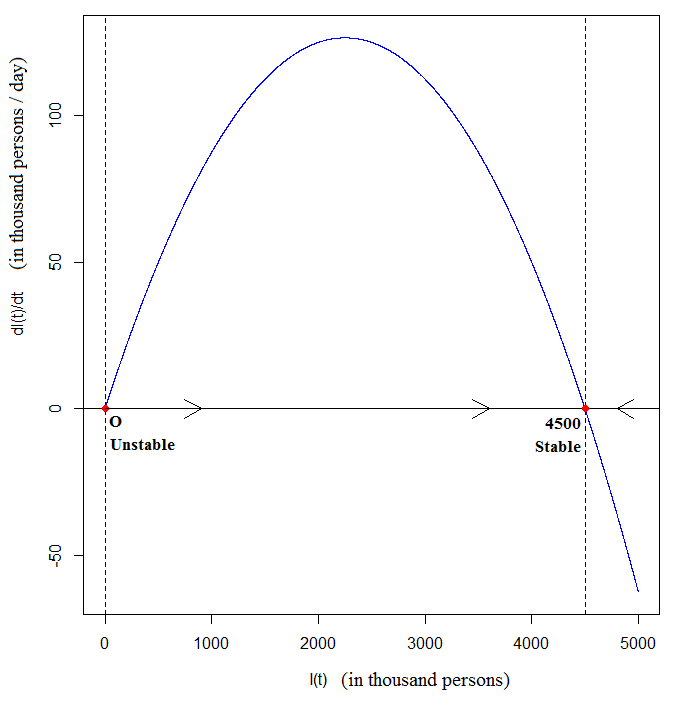
\includegraphics[width=\linewidth]{r1_2.png}
\caption{Equilibrium points at $I = 0$ and $I = 4500$ (in thousand persons)}
\label{fig:seq}
\end{figure}

\begin{figure}[H]
\centering
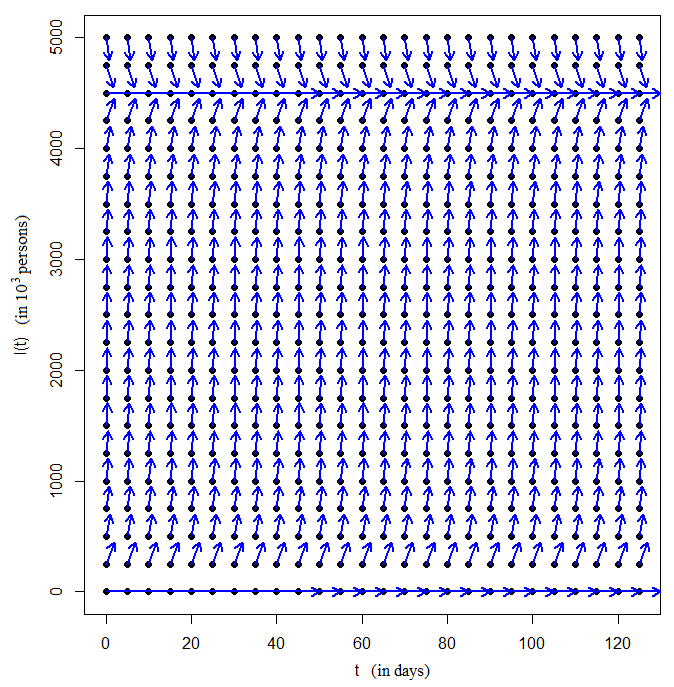
\includegraphics[width=\linewidth]{r1_1.png}
\caption{Direction Field for I(t)}
\label{fig:dir}
\end{figure}

\end{itemize}

\subsection{Numerical Solution with the Euler Method}
\label{subsection:euler}

The algorithm (taken from the course slides) shown in the following figure \ref{fig:euleralgo} will be used for numerical computation of the (equilibrium) solution using \textbf{Euler method}.

\begin{figure}[H]
\centering

\includegraphics[width=\linewidth]{algo.png}
\caption{Numerical Solution with Euler method \cite{bib:edx}}
\label{fig:euleralgo}
\end{figure}

\subsubsection{Finding the right step size (with $\beta=25 \times 10^{-6} / person /day$)} 

\begin{itemize}

\item In order to decide the best step size for the Euler method, first Euler method is run with different step sizes as shown in the figure \ref{fig:euler}. 

\item As can be seen from the following table \ref{table:diff} and the figure \ref{fig:euler}, the largest differences in the value of $I$ (with two consecutive step sizes) occurs around $78$ days:

\begin{table}[H]
  \begin{tabular}{ | c | c | c |  c | c | }
    \hline
    $\Delta t=1$ day &  & $\Delta t=0.5$ day &  & $\Delta t=0.25$ day \\ \hline
    I(78)=2220.351 &  & I(78)=2437.837 &  & I(78)=2546.591 \\ \hline
     & 217.487 & & 108.754 & \\ 
    \hline
  \end{tabular}
  \caption{Error in Euler method with different step sizes}
  \label{table:diff}
\end{table}

\begin{figure}[H]
\centering
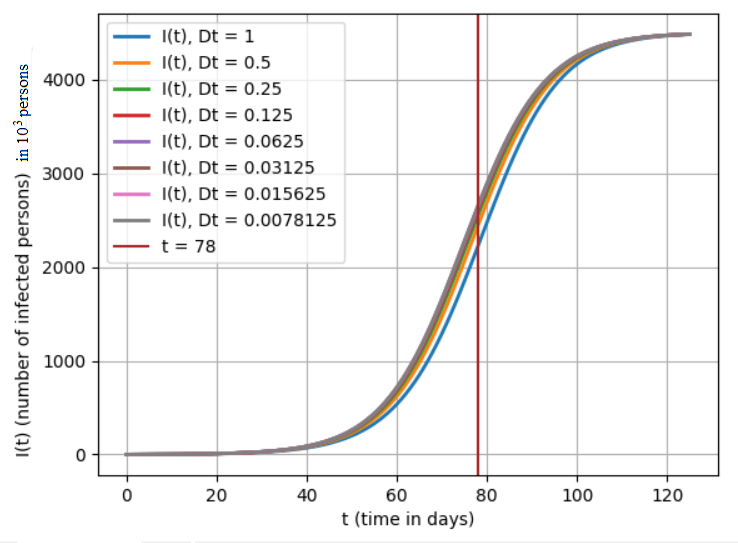
\includegraphics[width=\linewidth, height=12cm]{r1.png}
\caption{Solutions using different step sizes with Euler method (with $\beta=25 \times 10^{-6}$ /person /day)}
\label{fig:euler}
\end{figure}

\item As can be seen from the table in the \textit{Appendix B}, the first time when the error becomes $<1$ person (in thousands) is with the \textit{step size} $\frac{1}{512}$, hence this step size will be used for the \textit{Euler method}.


\end{itemize}

\subsubsection{Computing the (stable) equilibrium point}

\begin{itemize}

\item Now, this timestep will be used to solve the problem to find the equilibrium time $t_{eq}$ (in days). Find $t_{eq}$ such that $N-I(t_{eq})<\epsilon=10^{-6}$, the solution obtained is $t_{eq}=272.333984375$ days $\approx 273$ days.

\item Now, from the analytic solution \ref{eq:simsira} and the following figure \ref{fig:euleranl}, it can be verified that the $t_eq$ solution that the \textit{Euler method} obtained is pretty accurate (to the $\epsilon$ tolerance).

\begin{figure}[H]
\centering
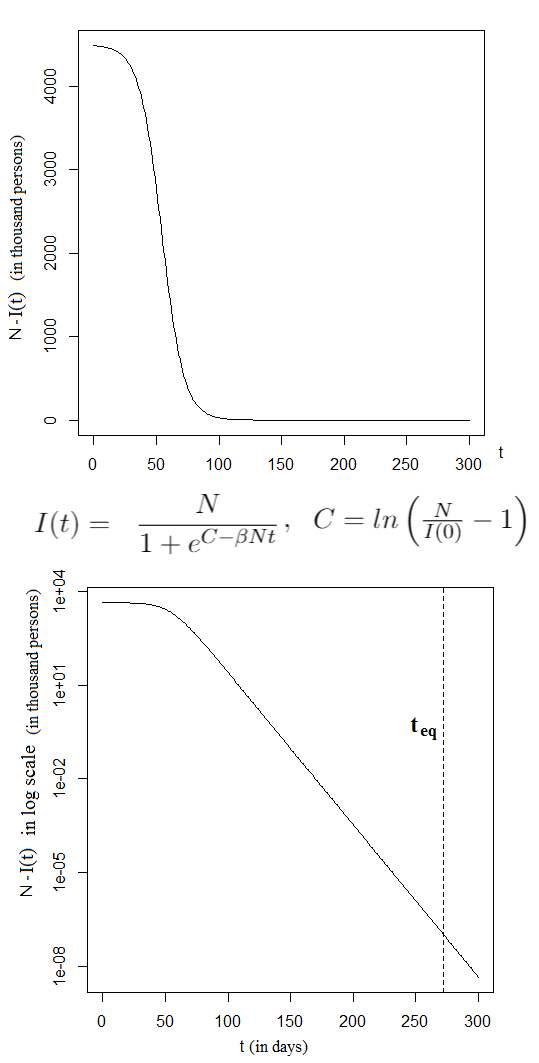
\includegraphics[width=\linewidth, height=20cm]{r2.png}
\caption{Comparing $t_{eq}$ obtained using Euler method with the analytic solution}
\label{fig:euleranl}
\end{figure}

\end{itemize}

\subsubsection{Results with $\beta=29 \times 10^{-6}$ / person / day, $I(0)=1$ person}

\begin{itemize}

 \item Following the same iterations as above, the steepest error is obtained at $t=67$ days in this case, as shown in the figure \ref{fig:euler1}.
 
 \item The first time when error becomes less than one person for $t=67$ days with Euler method is with step size $\frac{1}{512}$ again.
 
 \item The solution obtained is $t_{eq}=234.76953125$ days $\approx 235$ days, so the equilibrium (when \textbf{all} the population becomes \textbf{infected}) is obtained earlier as expected, since the \textbf{attack rate} $\beta$ is \textbf{higher}.

\begin{figure}[H]
\centering
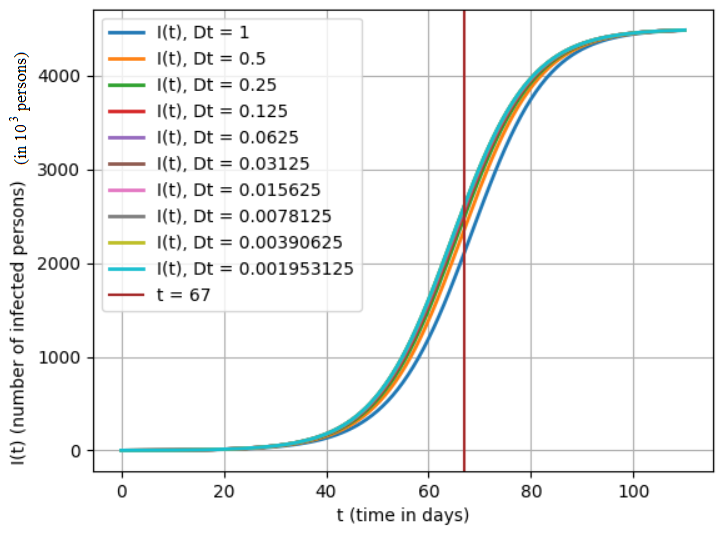
\includegraphics[width=\linewidth, height=12cm]{r1_3.png}
\caption{Solutions using different step sizes with Euler method (with $\beta=29 \times 10^{-6}$ / person / day)}
\label{fig:euler1}
\end{figure}

\end{itemize}

\subsubsection{Results with $\beta=25 \times 10^{-6}$ / person / day, with different initial values for infected persons ($I(0)$)}

\begin{itemize}

 \item Following the same iterations as above, the equilibrium point is computed using the Euler method with different values of initial infected population $I(0)$, as shown in the figure \ref{fig:euler1.1}.
 
 \item The solutions obtained are $t_{eq}=272.33, 258.02, 251.85, 248.23, 245.66,
 245.66$ days for $I(0)=1,5,10,15,20$ days, respectively. So the equilibrium is obtained earlier when the initial infected population size is higher, as expected.

\begin{figure}[H]
\centering
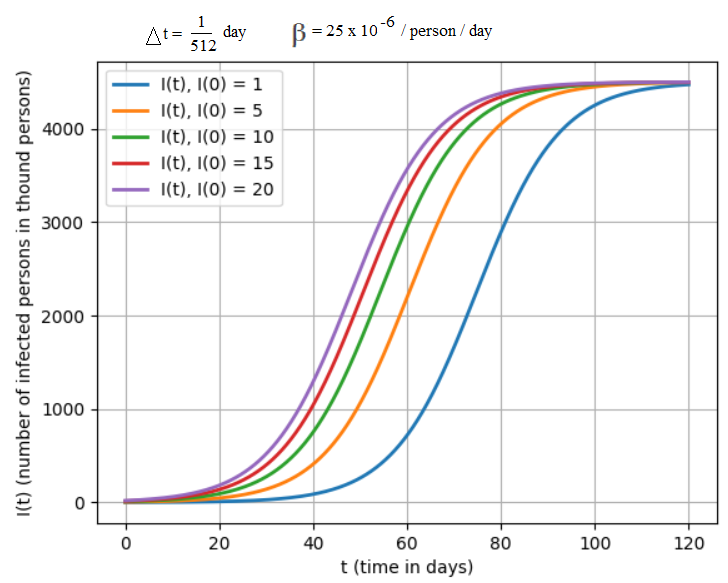
\includegraphics[width=\linewidth, height=12cm]{r1_4.png}
\caption{Solutions using different values of $I(0)$ with Euler method}
\label{fig:euler1.1}
\end{figure}

\end{itemize}

~
\newpage

\section{Simplified Model 2 (with $\beta=0$)}
\label{section:simplemathmodel2}

\begin{itemize}
\item Now let us assume that $\beta=0$ and that $\alpha>0$, so the flu can no more infect anyone (susceptible, if any, possibly because everyone got infected), an infected person recovers from flu with rate $\alpha$. This situation can be described again with a single differential equation in just $I(t)$ as shown in the equation below \ref{eq:simsir1}. 

\begin{equation}
\begin{array}{rcl} 
\dfrac{dI(t)}{dt} & = & -\alpha I(t)
\end{array}
\label{eq:simsir1}
\end{equation}


\item Also, let the the entire population be infected, $N=4500=I(0)$, (in thousand persons), \textit{initially} the number of persons \textit{susceptible} $=S(0)=0$, respectively. Let $\alpha=167 \times 10^{-3}$ (/ day) to start with.

\end{itemize}

\subsection{Analytic Solution}

\begin{itemize}

\item The analytic solution can be found by following the steps shown in the below equations \ref{eq:simsira1}:

\begin{equation}
\begin{array}{rcl} 
\dfrac{dI(t)}{dt} & = & -\alpha I(t) \\\\
\Rightarrow \int\limits_{I(0)}^{I(t)}\dfrac{dI(t)}{I(t)} & = & -\alpha \int\limits_{0}^{t}dt \\\\
\Rightarrow \left[ln|I(t)|\right]_{I(0)}^{I(t)}  & = & -\alpha [t]_{0}^{t} \\\\
\Rightarrow ln|I(t)|- ln|I(0)|  & = & -\alpha t \\\\
\Rightarrow I(t)  & = & I(0). e^{-\alpha t}
\end{array}
\label{eq:simsira1}
\end{equation}

\item The following figure \ref{fig:anl2} shows the \textbf{exponential} decay in $I(t)$ (\textbf{in thousand persons}) w.r.t. the time (\textbf{in days}) for different values of recovery rate $\alpha \times 10^{-3}$ (/ day). As expected, the higher the recovery rate, the quicker all the persons in the population get rid of the infection. 

\begin{figure}[H]
\centering
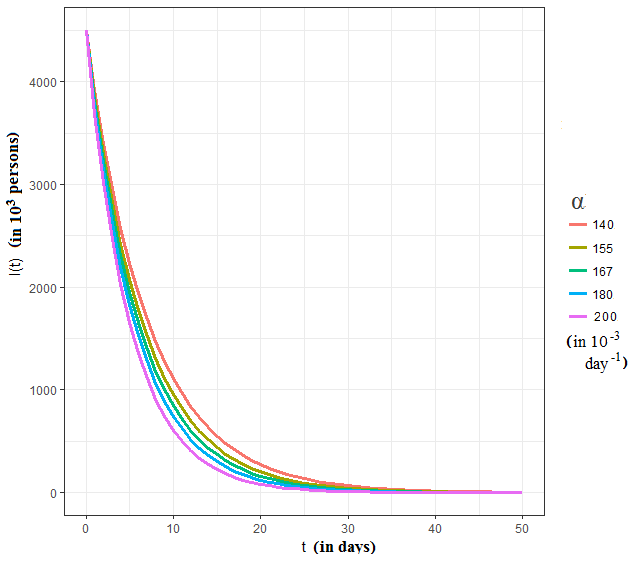
\includegraphics[width=\linewidth]{r3_0.png}
\caption{Decay of the number of infected persons}
\label{fig:anl2}
\end{figure}

\item Now, $I(t)+R(t)=N$ (since $S(t)=0$ forever, since no more infection) and $I(0)=N$, combining with the above analytic solution $I(t) = I(0).e^{-\alpha t} = N.e^{-\alpha t}$, we have, 

\begin{equation}
\begin{array}{rcl}
R(t) & = & N - I(t)  \\\\
     & = & N -  N.e^{-\alpha t} \\\\
\Rightarrow R(t) & = & N (1 - e^{-\alpha t})
\end{array}
\end{equation}

\item The following figure \ref{fig:anl3} shows the growth in $R(t)$ (\textbf{in thousand persons}) w.r.t. the time (\textbf{in days}) for different values of recovery rate $\alpha \times 10^{-3}$ (/ day). As expected, the higher the recovery rate, the quicker all the persons in the population move to the removed state. 

\begin{figure}[H]
\centering
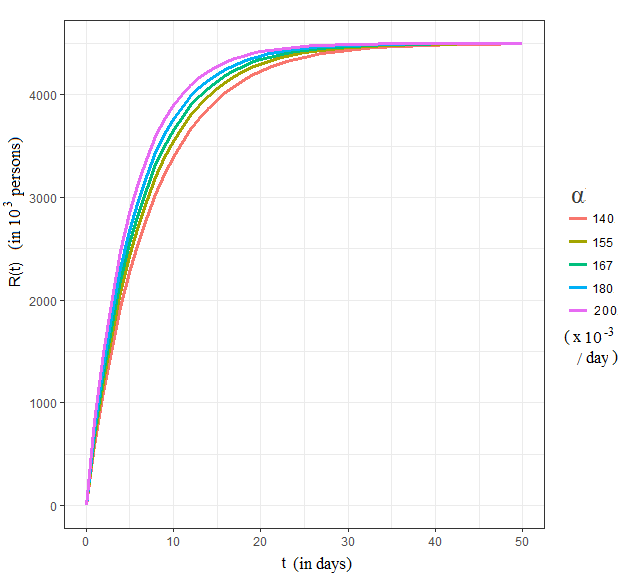
\includegraphics[width=\linewidth]{r3_01.png}
\caption{Growth of the number of recovered persons}
\label{fig:anl3}
\end{figure}

\end{itemize}

\subsection{Numerical Solution with the Euler Method}

\subsubsection{Solution with $\alpha=167 \times 10^{-3}$ / day}

\begin{itemize}
 
\item Following the same iterations as above, the steepest error is obtained at $t=6$ in this case, as shown in the figure \ref{fig:euler2}.
\item The first time when error becomes less than one person for $t=67$ with Euler method is with step size $\frac{1}{256}$.
\item The solution obtained with Euler method is $133.076171875$ days $\approx 133$ days to remove the infection from population with $10^{-6}$ tolerance. From the analytic solution, $I(133)= N.e^{-\alpha t} = 1.016478e-06$, similar result is obtained.

\subsubsection{Results}

The following figure \ref{fig:euler2} shows the solutions obtained with different step sizes using the Euler method. 

\begin{figure}[H]
\centering
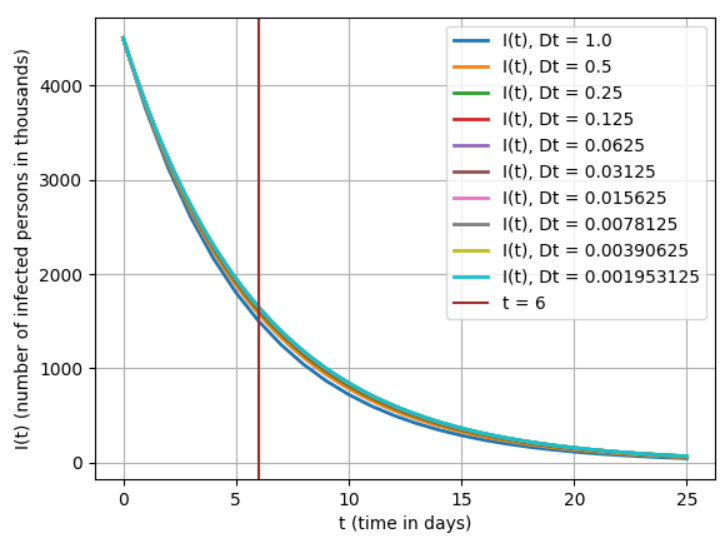
\includegraphics[width=\linewidth, height=12cm]{r3.png}
\caption{Solutions using different step sizes with Euler method (with $\alpha=167$ / day)}
\label{fig:euler2}
\end{figure}

\end{itemize}

\section{Generic Model (with $\alpha, \beta > 0$)}
\label{section:simplemathmodel2}

The following algorithm \ref{fig:euleralgo1} shown in the next figure is going to be used to obtain the solution using Euler method (the basic program for Euler's method, adapted to include three dependent variables and three differential equations).

\begin{figure}[H]
\centering
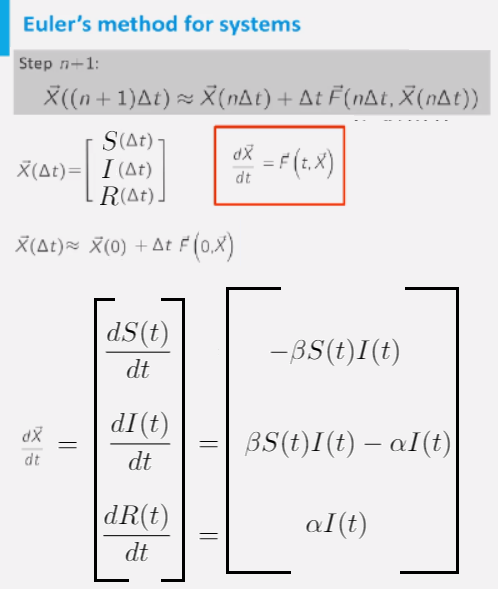
\includegraphics[width=\linewidth]{algo2.png}
\caption{Euler method for System of Differential Equations \cite{bib:edx}}
\label{fig:euleralgo1}
\end{figure}

\subsection{Equilibrium points}

\begin{itemize}

\item At the equilibrium point, $\dfrac{d\vec{X}}{dt}=0 \Rightarrow \dfrac{dS}{dt}=\dfrac{dI}{dt}=\dfrac{dR}{dt}=0 \Rightarrow I(t)=0$. There will be no infected person at the equilibrium point (infection should get removed).

\item As can be seen from the following figure \ref{fig:eq2} also, $I=0$ is an equilibrium point, which is quite expected, since in the equilibrium all the infected population will move to the \textit{removed state}. 

\item Also, at every point the invariant $S+I+R=N$ holds.

\item In this particular case shown in figure \ref{fig:eq2}, the susceptible population $S$ also becomes $0$ at equilibrium (since all the population got infected initially, all of them need to move to removed state) and $R=N=4500$ (in thousand persons). 

\end{itemize}


\begin{figure}[H]
\centering
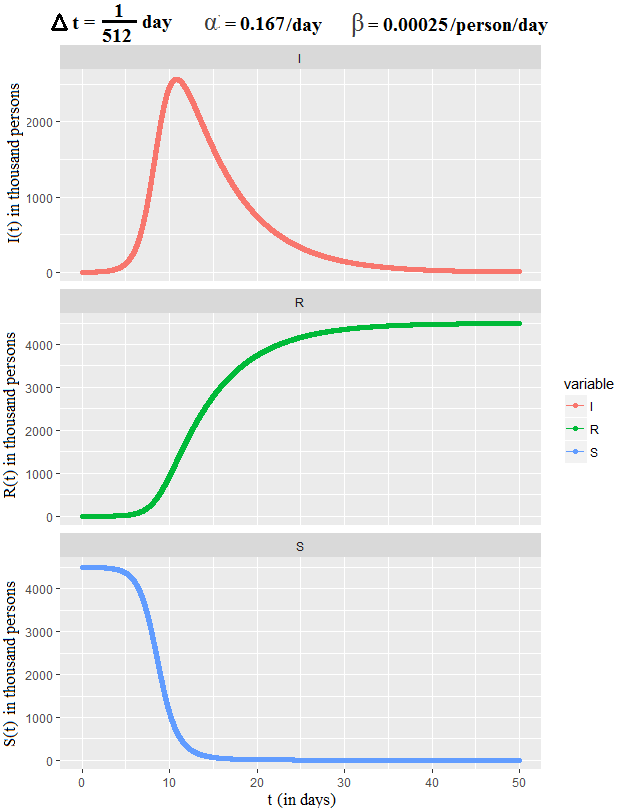
\includegraphics[width=\linewidth]{r4_3.png}
\caption{Equilibrium point $S=I=0$, $R=N$}
\label{fig:eq2}
\end{figure}


\subsection{Results with Euler method}

\begin{itemize}
\item As explained in the previous sections, the same iterative method is to find the right stepsize for the Euler method. The minimum of the two stepsizes determined is $\Delta t = \frac{1}{512}$ day and again this stepsize is going to be used for the Euler method.  

\item The following figures show the solutions obtained with different values of $\alpha, \beta$ with the initial infected population size $I(0)=1$ (in thousand persons). Higher values for the parameter $\beta$ obtained from the literature are used for simulation, since $\beta=25 \times 10^{-6}$ /person /day is too small (with the results not interesting) for the growth of the epidemic using the Euler method (at least till $\Delta t=\frac{1}{2^15}$, after which the iterative Euler method becomes very slow).

\item As can be seen, from the figures \ref{fig:euler2}, \ref{fig:euler3} and \ref{fig:euler4}, at equilibrium, $I$ becomes zero. 

\item The solution (number of days to reach equilibrium) obtained at $\alpha=167 \times 10^{-3}$ /day and $\beta=25 \times 10^{-5}$ /person /day is $t_{eq}=143.35546875 \approx 144$ days with $I(0)=1$  (in thousand persons), the corresponding figure is figure \ref{fig:euler2}. 

\item The solution (number of days to reach equilibrium) obtained at $\alpha=167 \times 10^{-3}$ /day and $\beta=5 \times 10^{-5}$ /person /day is $t_{eq} \approx 542$ days with $I(0)=1$  (in thousand persons), the corresponding figure is figure \ref{fig:euler3}. Hence, higher the $\beta$ value, the equilibrium is reached much earlier. 

\item The solution obtained at $\alpha=500 \times 10^{-3}$ /day and $\beta=25 \times 10^{-5}$ /person /day is $t_{eq} \approx 78$ days with $I(0)=1$  (in thousand persons), the corresponding figure is figure \ref{fig:euler4}. Hence, higher the $\alpha$ value, the equilibrium is reached earlier. 

\item The solution obtained at $\alpha=167 \times 10^{-3}$ /day and $\beta=25 \times 10^{-5}$ /person /day is $t_{eq}=140$ days with $I(0)=10$. Hence, as expected, higher the number of initial infected population size, quicker the equilibrium is reached.

\item At equilibrium, $S$ does not necessarily become zero, since sometimes the entire population may  not get infected ever, as shown in the figure \ref{fig:euler3}, where at equilibrium the susceptible population is non-zero. 

\begin{figure}[H]
\centering
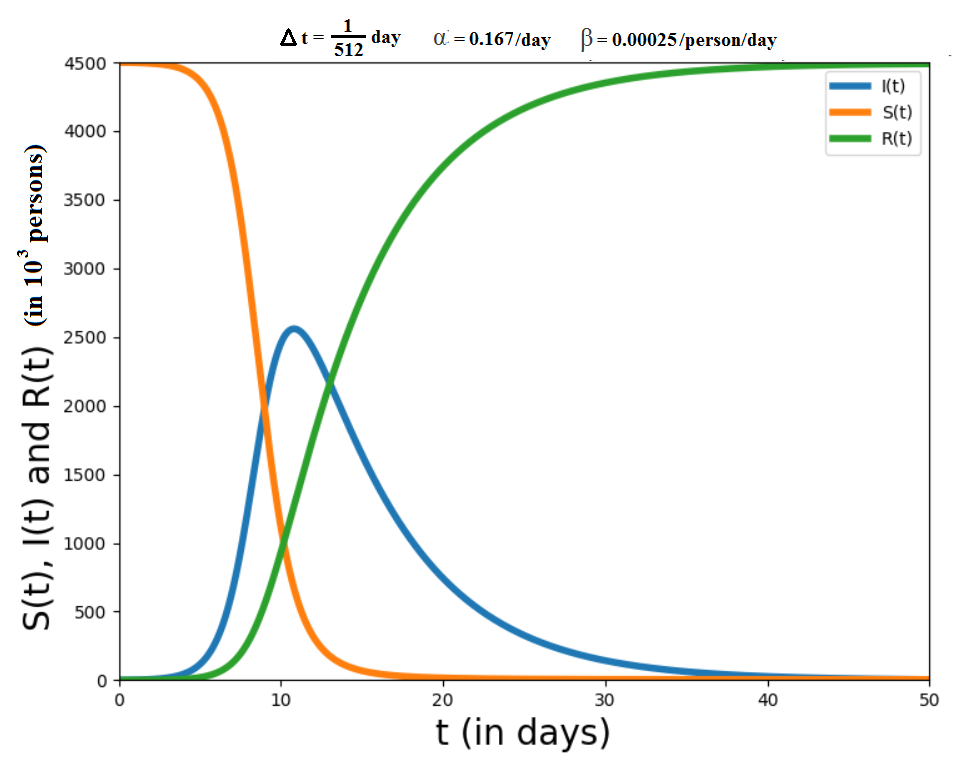
\includegraphics[width=\linewidth, height=12cm]{r4.png}
\caption{Numerical Solution with Euler method}
\label{fig:euler2}
\end{figure}

\begin{figure}[H]
\centering
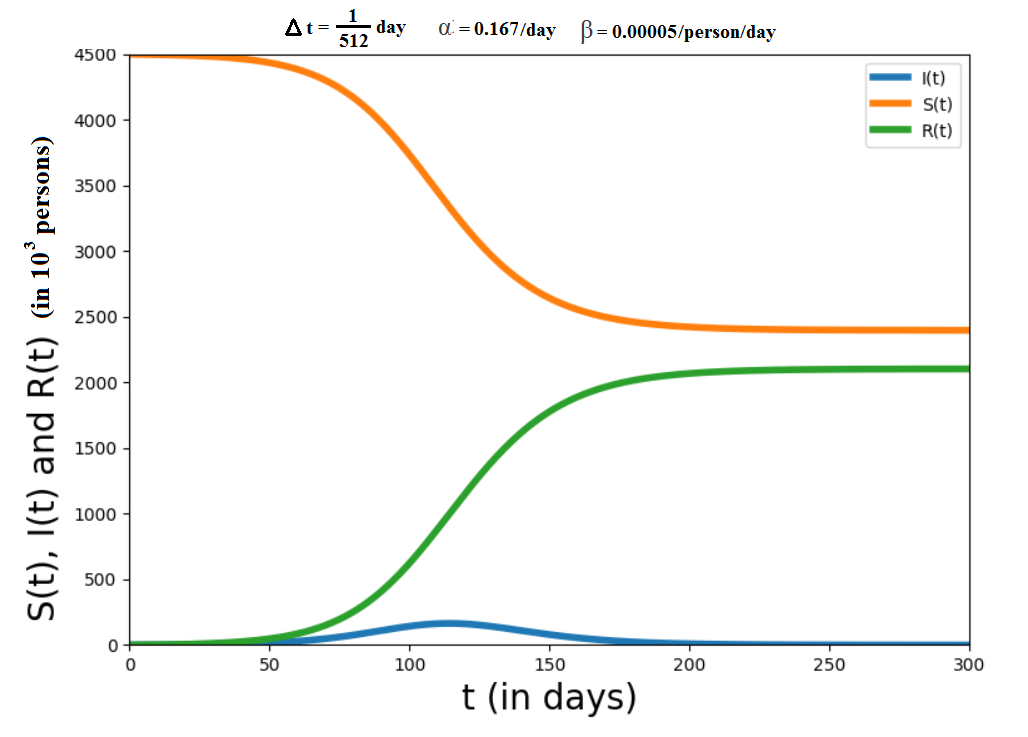
\includegraphics[width=\linewidth, height=12cm]{r4_0.png}
\caption{Numerical Solution with Euler method}
\label{fig:euler3}
\end{figure}

\begin{figure}[H]
\centering
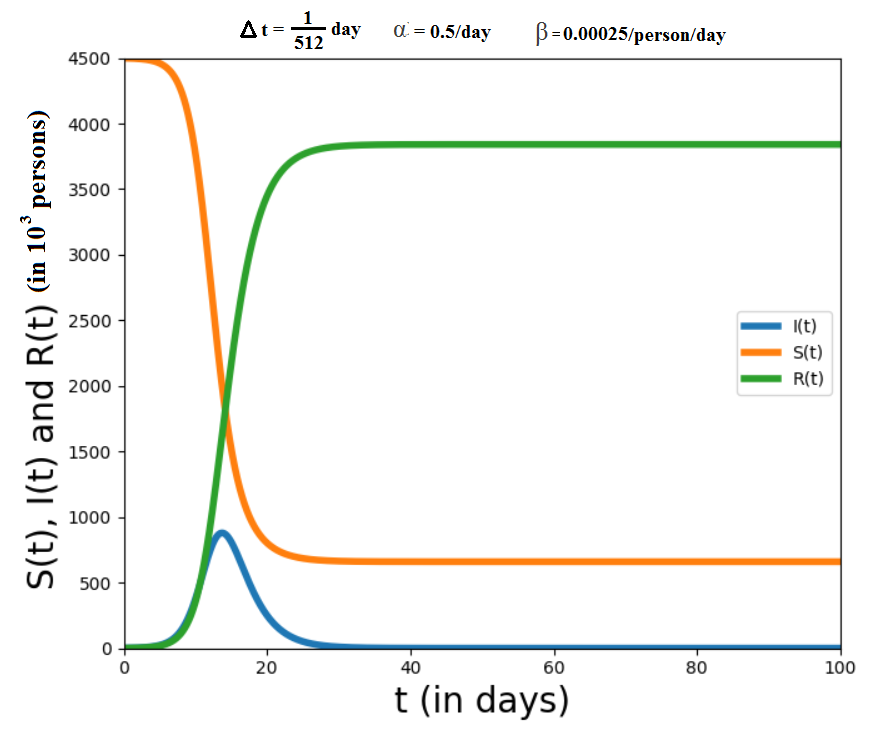
\includegraphics[width=\linewidth, height=12cm]{r4_4.png}
\caption{Numerical Solution with Euler method}
\label{fig:euler4}
\end{figure}

\begin{figure}[H]
\centering
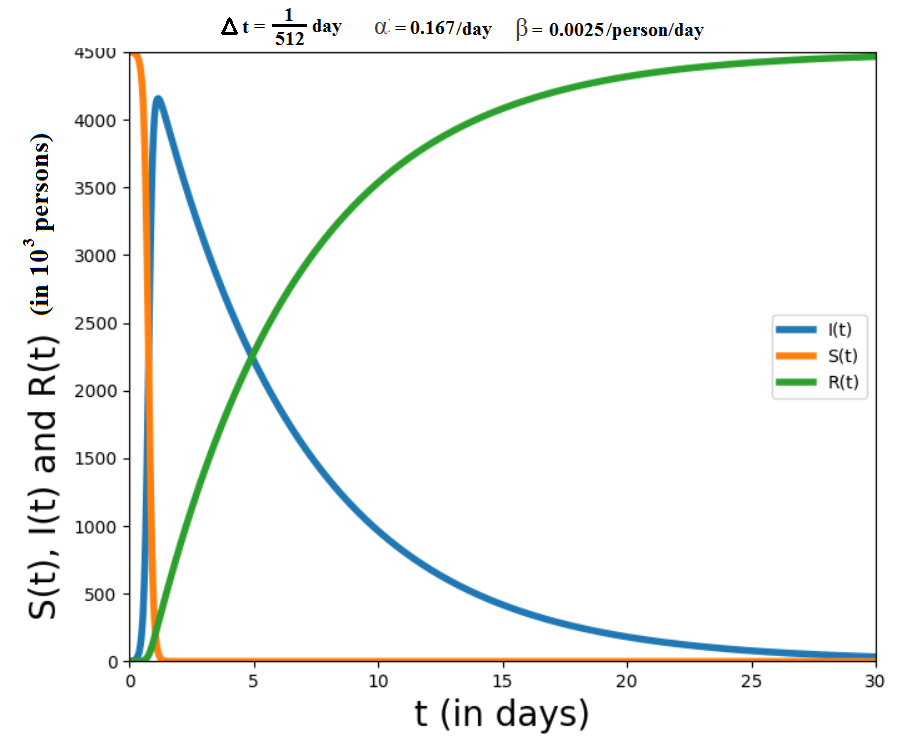
\includegraphics[width=\linewidth, height=12cm]{r4_01.png}
\caption{Numerical Solution with Euler method}
\label{fig:euler4}
\end{figure}

\item As can be seen from the phase planes from following figure \ref{fig:euler5}, at equilibrium, the infected population becomes $0$. 

\begin{figure}[H]
\centering
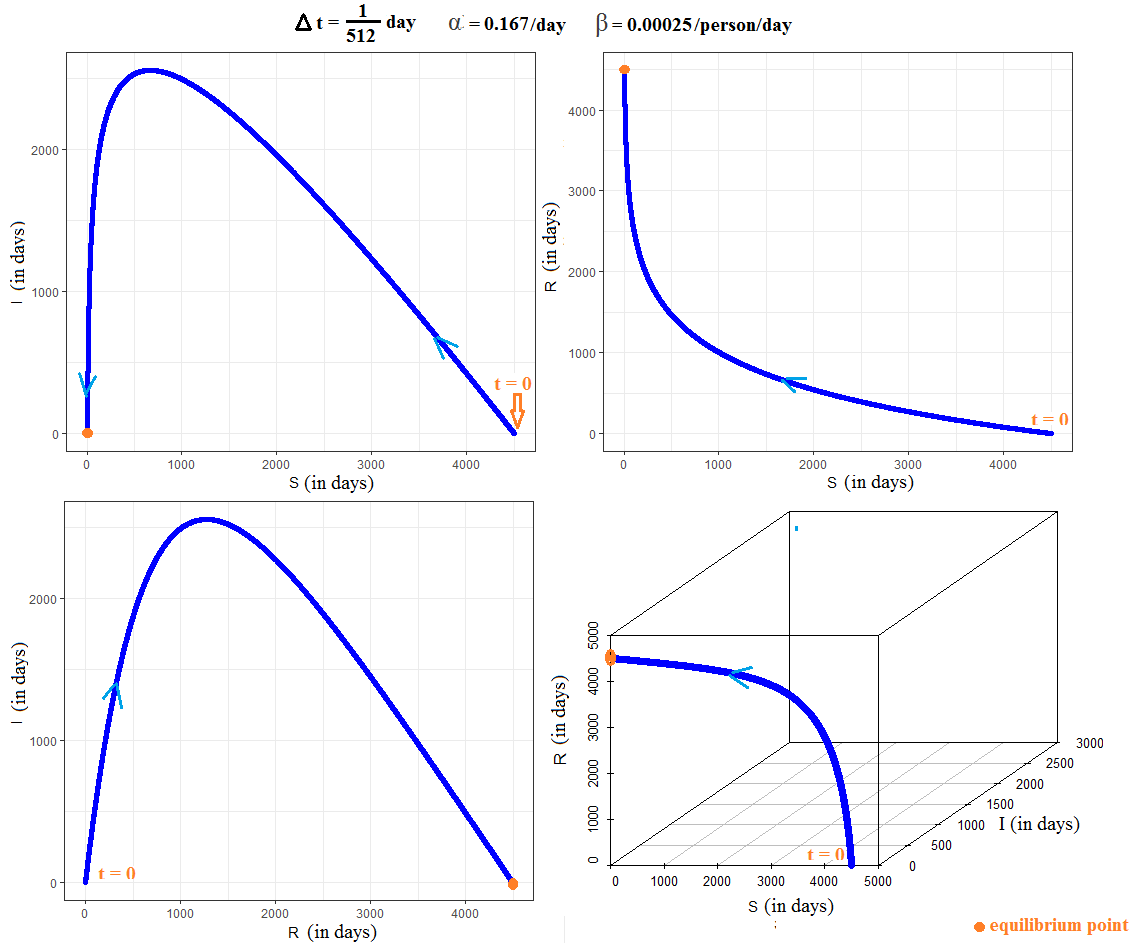
\includegraphics[width=\linewidth, height=15cm]{r4_1.png}
\caption{Phase planes for the generic model}
\label{fig:euler5}
\end{figure}

\end{itemize}

\chapter{Conclusions} 
In this report, the spread of the pandemic influenza A (H1N1) that had an outbreak in Kolkata, West Bengal, India, 2010 was simulated using the basic epidemic SIR model.Initially there will be a small number of infected persons in the population, most of the population had susceptible persons (still not infected but prone to be infected) and zero removed persons. Given the initial values of the variables and the parameter (attack and recovery rates of the flu) values, the following questions were attempted to be answered with the simulation / analysis:

\begin{enumerate}
\item Whether the number of infected persons increase substantially, producing an epidemic, or the flue will fizzle out. 
\item Assuming there is an epidemic, how will it end? Will there still be any susceptibles left when it is over? 
\item How long will the epidemic last?
\end{enumerate}

The following conclusions are obtained after running the simulations with different values of the parameters and the initial values of the variables:

\begin{enumerate}
\item When the recovery rate $\alpha$ is $\approx 0$ or very low compared to the attack rate $\beta$, the flu will turn out to be an epidemic and the entire population will be infected first (the higher $\beta$ is the quicker the epidemic). 
\item When there is an epidemic, it will eventually end in the equilibrium point with $0$ infected population, how fast it reaches the equilibrium depends upon the recovery rate (the higher $\alpha$ is the quicker the infection removal).
\item The time to reach the equilibrium can be computed using Euler method, it depends on the parameters $\alpha$ (the higher the quicker) and $\beta$ (the higher the quicker) and the initial infected populated size $I(0)$ (the higher the quicker).
\item If there the recovery rate $\alpha$ is higher than the attack rate  $\beta$, even when the equilibrium is reached the susceptible population size may be non-zero. 
\end{enumerate}

\begin{thebibliography}{10}  % This number indicates the number of symbols in the maximum number of items in the bibliography
\addcontentsline{toc}{chapter}{Bibliography} %Adds a line to table of contents

\bibitem{bib:wiki} \textit{Swine influenza}, 
Wikipedia, 
the free encyclopedia, 
\url{https://en.wikipedia.org/wiki/Swine_influenza}. 

\bibitem{bib:ijmr} An outbreak of pandemic influenza A (H1N1) in Kolkata, 
West Bengal, 
India, 
2010,
\url{https://www.ncbi.nlm.nih.gov/pmc/articles/PMC3385238/}.

\bibitem{bib:virus} Electron microscope image of the re-assorted H1N1 influenza virus photographed at the CDC Influenza Laboratory,
\url{https://www.cdc.gov/h1n1flu/images/B00528_H1N1_flu_blue_sml.jpg}.

\bibitem{bib:kmc} Basic Statistics, 
Kolkata Municipal Corporation,
\url{https://www.kmcgov.in/KMCPortal/jsp/BasicStatistics.jsp}.

\bibitem{bib:edx} DelftX: MathMod1x Mathematical Modelling Basics,
edX online course,
week2 and week3 lecture videos, 
\url{https://courses.edx.org/courses/course-v1:DelftX+MathMod1x+2T2017/}

\end{thebibliography}  

\appendix     
\chapter{Analytic derivation of the solution of the simplified SIR Model1 ($\alpha=0$)} 

\begin{equation*}
\begin{array}{rcl} 
\dfrac{dI(t)}{dt} & = & \beta I(t)(N-I(t)) \\\\
\Rightarrow \int\limits_{I(0)}^{I(t)}\dfrac{dI(t)}{I(t)(N-I(t))} & = & \beta \int\limits_{0}^{t}dt \\\\
\Rightarrow \frac{1}{N}\left(\int\limits_{I(0)}^{I(t)}\dfrac{dI(t)}{I(t)} + \int\limits_{I(0)}^{I(t)}\dfrac{dI(t)}{N-I(t)}\right) & = & \beta \int\limits_{0}^{t}dt \\\\
\Rightarrow \left[ln|I(t)|\right]_{I(0)}^{I(t)} + \left[-ln|N-I(t)|\right]_{I(0)}^{I(t)} & = & \beta N [t]_{0}^{t} \\\\
\Rightarrow ln\frac{I(t)}{N-I(t)} + ln\left(\frac{N}{I(0)}-1\right) & = & \beta N t, \;\;\;\; 0 \leq I(t) \leq N\\\\
\Rightarrow ln\frac{I(t)}{N-I(t)} & = & \beta N t - C, \;\;\;\;  C = ln\left(\frac{N}{I(0)}-1\right)\; (let)\\\\
\Rightarrow I(t)  & = & \dfrac{N}{1+e^{C-\beta N t}}
\end{array}
\end{equation*}

\chapter{Error table for Euler method} 

\begin{table*}[h!]
  \begin{tabular}{ | c | c | }
    \hline
    $\Delta t$ (in day) &  Error=$E_{\Delta t}=y(t)-w_{\Delta t} \approx w_{\Delta t}-w_{2\Delta t}$ (in thousand persons) \\ \hline
    $\frac{1}{2}$   &    217.486594639 \\ \hline
    $\frac{1}{4}$   &    108.754179087 \\ \hline
    $\frac{1}{8}$   &    54.0574495747 \\ \hline
    $\frac{1}{16}$   &    26.9092982076 \\ \hline
    $\frac{1}{32}$  &    13.4199659856 \\ \hline
    $\frac{1}{64}$  &    6.70071788053 \\ \hline
    $\frac{1}{128}$  &    3.3479689886 \\ \hline
    $\frac{1}{256}$ &    1.67337783755 \\ \hline
    $\frac{1}{512}$ &    0.83653611108 \\ \hline
    \hline
  \end{tabular}
%  \caption{Finding the right step size for Euler method}
\end{table*}

\end{document}